% Options for packages loaded elsewhere
% Options for packages loaded elsewhere
\PassOptionsToPackage{unicode}{hyperref}
\PassOptionsToPackage{hyphens}{url}
\PassOptionsToPackage{dvipsnames,svgnames,x11names}{xcolor}
%
\documentclass[
  spanish,
  letterpaper,
  DIV=11,
  numbers=noendperiod]{scrartcl}
\usepackage{xcolor}
\usepackage{amsmath,amssymb}
\setcounter{secnumdepth}{-\maxdimen} % remove section numbering
\usepackage{iftex}
\ifPDFTeX
  \usepackage[T1]{fontenc}
  \usepackage[utf8]{inputenc}
  \usepackage{textcomp} % provide euro and other symbols
\else % if luatex or xetex
  \usepackage{unicode-math} % this also loads fontspec
  \defaultfontfeatures{Scale=MatchLowercase}
  \defaultfontfeatures[\rmfamily]{Ligatures=TeX,Scale=1}
\fi
\usepackage{lmodern}
\ifPDFTeX\else
  % xetex/luatex font selection
\fi
% Use upquote if available, for straight quotes in verbatim environments
\IfFileExists{upquote.sty}{\usepackage{upquote}}{}
\IfFileExists{microtype.sty}{% use microtype if available
  \usepackage[]{microtype}
  \UseMicrotypeSet[protrusion]{basicmath} % disable protrusion for tt fonts
}{}
\makeatletter
\@ifundefined{KOMAClassName}{% if non-KOMA class
  \IfFileExists{parskip.sty}{%
    \usepackage{parskip}
  }{% else
    \setlength{\parindent}{0pt}
    \setlength{\parskip}{6pt plus 2pt minus 1pt}}
}{% if KOMA class
  \KOMAoptions{parskip=half}}
\makeatother
% Make \paragraph and \subparagraph free-standing
\makeatletter
\ifx\paragraph\undefined\else
  \let\oldparagraph\paragraph
  \renewcommand{\paragraph}{
    \@ifstar
      \xxxParagraphStar
      \xxxParagraphNoStar
  }
  \newcommand{\xxxParagraphStar}[1]{\oldparagraph*{#1}\mbox{}}
  \newcommand{\xxxParagraphNoStar}[1]{\oldparagraph{#1}\mbox{}}
\fi
\ifx\subparagraph\undefined\else
  \let\oldsubparagraph\subparagraph
  \renewcommand{\subparagraph}{
    \@ifstar
      \xxxSubParagraphStar
      \xxxSubParagraphNoStar
  }
  \newcommand{\xxxSubParagraphStar}[1]{\oldsubparagraph*{#1}\mbox{}}
  \newcommand{\xxxSubParagraphNoStar}[1]{\oldsubparagraph{#1}\mbox{}}
\fi
\makeatother


\usepackage{longtable,booktabs,array}
\usepackage{calc} % for calculating minipage widths
% Correct order of tables after \paragraph or \subparagraph
\usepackage{etoolbox}
\makeatletter
\patchcmd\longtable{\par}{\if@noskipsec\mbox{}\fi\par}{}{}
\makeatother
% Allow footnotes in longtable head/foot
\IfFileExists{footnotehyper.sty}{\usepackage{footnotehyper}}{\usepackage{footnote}}
\makesavenoteenv{longtable}
\usepackage{graphicx}
\makeatletter
\newsavebox\pandoc@box
\newcommand*\pandocbounded[1]{% scales image to fit in text height/width
  \sbox\pandoc@box{#1}%
  \Gscale@div\@tempa{\textheight}{\dimexpr\ht\pandoc@box+\dp\pandoc@box\relax}%
  \Gscale@div\@tempb{\linewidth}{\wd\pandoc@box}%
  \ifdim\@tempb\p@<\@tempa\p@\let\@tempa\@tempb\fi% select the smaller of both
  \ifdim\@tempa\p@<\p@\scalebox{\@tempa}{\usebox\pandoc@box}%
  \else\usebox{\pandoc@box}%
  \fi%
}
% Set default figure placement to htbp
\def\fps@figure{htbp}
\makeatother



\ifLuaTeX
\usepackage[bidi=basic]{babel}
\else
\usepackage[bidi=default]{babel}
\fi
% get rid of language-specific shorthands (see #6817):
\let\LanguageShortHands\languageshorthands
\def\languageshorthands#1{}


\setlength{\emergencystretch}{3em} % prevent overfull lines

\providecommand{\tightlist}{%
  \setlength{\itemsep}{0pt}\setlength{\parskip}{0pt}}



 


\KOMAoption{captions}{tableheading}
\makeatletter
\@ifpackageloaded{caption}{}{\usepackage{caption}}
\AtBeginDocument{%
\ifdefined\contentsname
  \renewcommand*\contentsname{Tabla de contenidos}
\else
  \newcommand\contentsname{Tabla de contenidos}
\fi
\ifdefined\listfigurename
  \renewcommand*\listfigurename{Listado de Figuras}
\else
  \newcommand\listfigurename{Listado de Figuras}
\fi
\ifdefined\listtablename
  \renewcommand*\listtablename{Listado de Tablas}
\else
  \newcommand\listtablename{Listado de Tablas}
\fi
\ifdefined\figurename
  \renewcommand*\figurename{Figura}
\else
  \newcommand\figurename{Figura}
\fi
\ifdefined\tablename
  \renewcommand*\tablename{Tabla}
\else
  \newcommand\tablename{Tabla}
\fi
}
\@ifpackageloaded{float}{}{\usepackage{float}}
\floatstyle{ruled}
\@ifundefined{c@chapter}{\newfloat{codelisting}{h}{lop}}{\newfloat{codelisting}{h}{lop}[chapter]}
\floatname{codelisting}{Listado}
\newcommand*\listoflistings{\listof{codelisting}{Listado de Listados}}
\makeatother
\makeatletter
\makeatother
\makeatletter
\@ifpackageloaded{caption}{}{\usepackage{caption}}
\@ifpackageloaded{subcaption}{}{\usepackage{subcaption}}
\makeatother
\usepackage{bookmark}
\IfFileExists{xurl.sty}{\usepackage{xurl}}{} % add URL line breaks if available
\urlstyle{same}
\hypersetup{
  pdftitle={Cecilia: una familia de modelos de lenguaje continual-pretrained en español cubano},
  pdfauthor={Equipo Cecilia --- GIA-UH / GPLSI / Syalia},
  pdflang={es},
  colorlinks=true,
  linkcolor={blue},
  filecolor={Maroon},
  citecolor={Blue},
  urlcolor={Blue},
  pdfcreator={LaTeX via pandoc}}


\title{Cecilia: una familia de modelos de lenguaje continual-pretrained
en español cubano}
\author{Equipo Cecilia --- GIA-UH / GPLSI / Syalia}
\date{2026-04-21}
\begin{document}
\maketitle


\subsection{1. Resumen}\label{resumen}

\textbf{Cecilia}\footnote{El reporte técnico extendido en inglés se
  encuentra en \texttt{report/report.md}; el paper académico en formato
  LNCS, en \texttt{papers/uciencia25/paper.pdf}.} es una familia de
modelos de lenguaje \emph{continual-pretrained} en español cubano,
desarrollada por el Grupo de Inteligencia Artificial de la Universidad
de La Habana (GIA-UH), en colaboración con el Grupo de Procesamiento del
Lenguaje y Sistemas de Información (GPLSI) de la Universidad de
Alicante, y con apoyo de Syalia y Epistemial. La primera versión
liberada, \textbf{Cecilia 2B v0.1}, adapta el modelo base
\textbf{Salamandra 2B} mediante \emph{continual pretraining} sobre
aproximadamente mil millones de tokens de texto cubano: prensa, EcuRed,
leyes, literatura y lírica. Sobre esa base se publicaron también una
variante \emph{instruction-tuned} (\texttt{cecilia-2b-instruct-v1}) y su
correspondiente versión cuantizada en formato GGUF.

\subsection{2. Arquitectura del modelo}\label{arquitectura-del-modelo}

Cecilia 2B se construye sobre \textbf{Salamandra 2B}, un
\emph{transformer} decoder-only desarrollado por el Barcelona
Supercomputing Center, con 24 capas, \emph{hidden size} 2048, 16
\emph{attention heads}, y aproximadamente 2.25 mil millones de
parámetros. La arquitectura incorpora \emph{rotary positional
embeddings} (RoPE), activaciones SwiGLU, normalización RMS y \emph{flash
attention}; el vocabulario es de 256K tokens y la ventana de contexto,
de 8192 tokens.

La adaptación al español cubano se realiza \textbf{exclusivamente vía
continual pretraining}: ni la arquitectura ni el tokenizador ni el
vocabulario se modifican. Esta decisión preserva las capacidades
multilingües del modelo base y evita introducir variabilidad no
atribuible al corpus, pero implica que cubanismos y términos
transliterados fuera del vocabulario de Salamandra reciben una
tokenización subóptima --- limitación reconocida y abordada en la
sección 7.

La elección de Salamandra como base responde a tres criterios: foco
multilingüe con énfasis explícito en español y co-oficiales, licencia
Apache 2.0 que permite redistribución académica y comercial, y un tamaño
compatible con despliegue en hardware modesto, condición relevante para
los entornos de cómputo típicos en Cuba.

\subsection{3. Corpus y pipeline de
datos}\label{corpus-y-pipeline-de-datos}

El corpus de entrenamiento agrupa \textbf{296,311 archivos},
\textbf{\textasciitilde2,631 millones de caracteres} y
\textbf{\textasciitilde385 millones de palabras}, distribuidos en
aproximadamente 3000 dominios. Las fuentes principales son: la prensa
cubana de la última década (Granma, Juventud Rebelde --- pipelines en
\texttt{data/granma/}, \texttt{data/jr/}); la enciclopedia colaborativa
\textbf{EcuRed} (\texttt{data/ecured/}), dominante en número de
archivos; una compilación de \textbf{leyes cubanas}; alrededor de 400
obras literarias cubanas; enciclopedias locales documentando cubanismos;
y letras de canciones populares. Toda la recolección se hizo bajo
asunción de \emph{fair use} estrictamente para investigación académica;
el corpus crudo no se redistribuye.

Tras tokenización con el \emph{tokenizer} original de Salamandra, el
corpus se materializa en \textbf{1,104,532 muestras} y
\textbf{982,024,795 tokens efectivos} (sin \emph{padding}) ---
1,131,040,768 con \emph{padding}, ratio de \emph{padding} del 13.2\%. La
longitud media de secuencia es de 889 tokens y la segmentación final
produjo \textbf{959,008 ventanas de contexto} de 1024 tokens. La
densidad léxica de 6.8 caracteres por palabra y la longitud media de
documento de \textasciitilde8,900 caracteres reflejan una mezcla
balanceada entre textos breves (entradas enciclopédicas cortas, lírica)
y narrativos largos (literatura, leyes).

\begin{figure}

\centering{

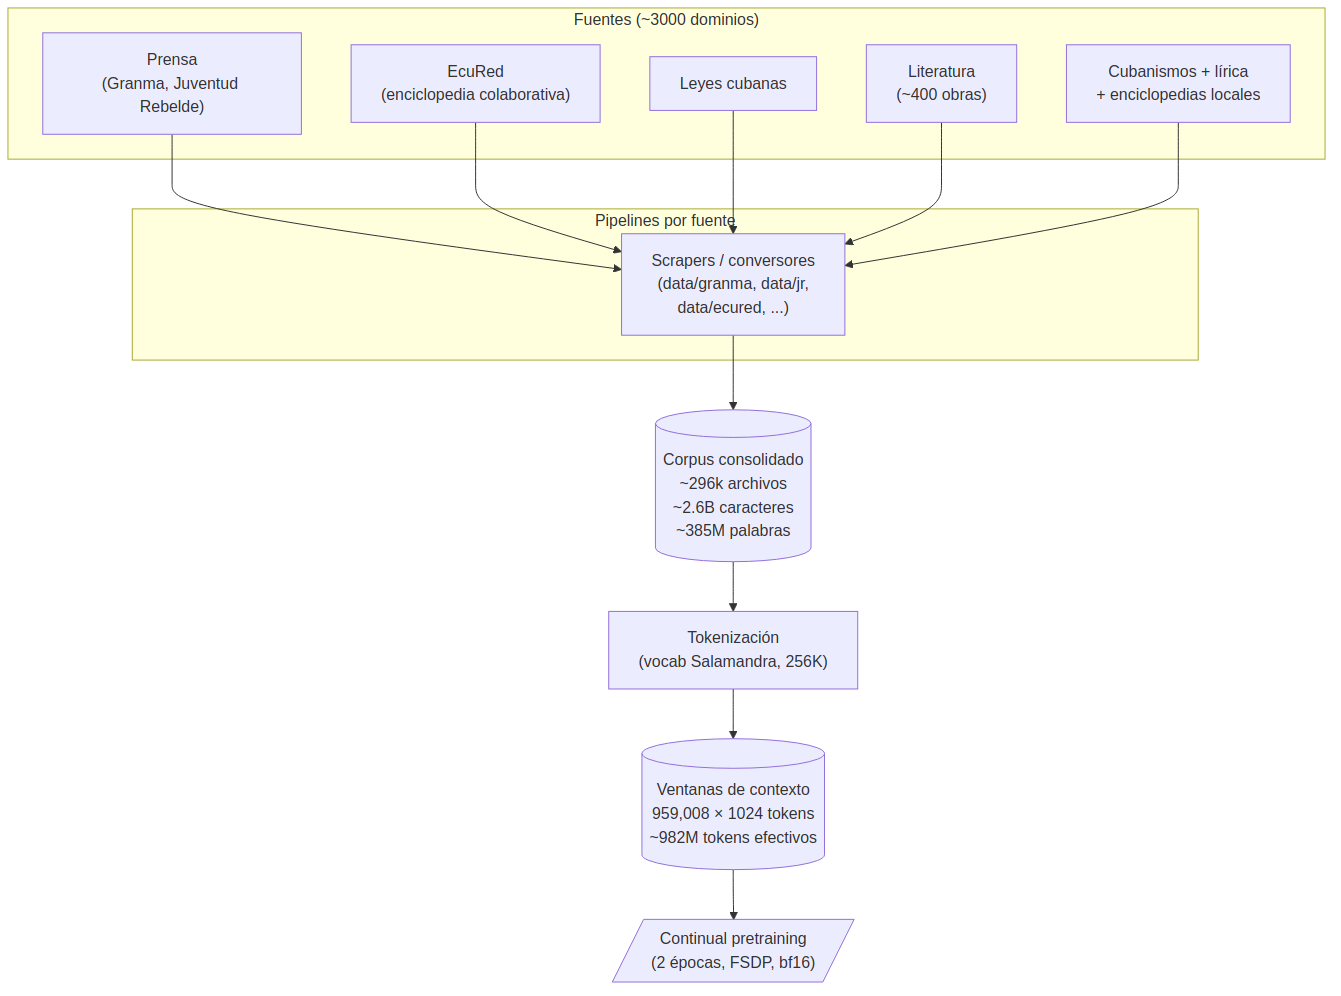
\includegraphics[width=0.8\linewidth,height=\textheight,keepaspectratio]{figs/pipeline-datos.png}

}

\caption{\label{fig-pipeline-datos}Pipeline de datos: fuentes
heterogéneas, pipelines específicos por fuente, consolidación,
tokenización y entrenamiento.}

\end{figure}%

\subsection{4. Procedimiento de continual
pretraining}\label{procedimiento-de-continual-pretraining}

El entrenamiento se ejecutó por \textbf{dos épocas completas} sobre el
corpus tokenizado, con \emph{batch size} de 4 y \emph{gradient
accumulation} de 16 pasos, equivalente a un \emph{batch} efectivo de 64.
La optimización usó \textbf{AdamW} con \emph{learning rate} 2e-5,
\emph{weight decay} 0.01, betas (0.9, 0.999), y \emph{gradient clipping}
a norma 1.0. El \emph{scheduler} siguió un esquema \emph{warmup-linear}
con 6\% de \emph{warmup} --- fracción deliberadamente pequeña, ya que en
\emph{continual pretraining} el modelo parte de un estado convergente y
no requiere el \emph{warmup} extendido típico del entrenamiento desde
cero.

La precisión empleada fue \textbf{bfloat16} mixta, con paralelización
\textbf{FSDP} (\emph{full sharding} y \emph{sharded state dicts}) y
\emph{gradient checkpointing} activado para reducir el \emph{footprint}
de memoria a costa de cómputo adicional en el \emph{backward pass}. La
validación se ejecutó tras cada época y, adicionalmente, cada 640 pasos
de entrenamiento, para detectar tempranamente regresiones o
inestabilidad.

El cómputo se realizó sobre \textbf{2 × NVIDIA A100 (40 GB)} acompañadas
por un AMD EPYC con 128 \emph{cores} y 1 TB de RAM. La duración total
del entrenamiento fue de aproximadamente \textbf{48 horas}.

\begin{longtable}[]{@{}ll@{}}
\toprule\noalign{}
Parámetro & Valor \\
\midrule\noalign{}
\endhead
\bottomrule\noalign{}
\endlastfoot
Épocas & 2 \\
Batch size & 4 \\
Gradient accumulation & 16 \\
Batch efectivo & 64 \\
Optimizador & AdamW \\
Learning rate & 2e-5 \\
Weight decay & 0.01 \\
Warmup proportion & 6\% \\
Precisión & bfloat16 \\
Paralelización & FSDP (full sharding) \\
\end{longtable}

\subsection{5. Evaluación y
trade-offs}\label{evaluaciuxf3n-y-trade-offs}

La evaluación comparativa contra el modelo base Salamandra 2B se ejecutó
sobre una batería estándar de \emph{benchmarks} generales en inglés y
español: ARC, BELEBELE, OpenBookQA, PAWS, PIQA, SocialIQA, XNLI,
XStoryCloze, XQuAD, TriviaQA, XLSum, Cocoteros, ESCOLA, TECA y WNLI. La
diferencia agregada relativa al base es de \textbf{−2.4\%} en promedio
sobre todas las tareas. La tabla siguiente resume las principales
mejoras y regresiones; los detalles completos viven en
\texttt{report/report.md}.

\begin{longtable}[]{@{}llrrr@{}}
\toprule\noalign{}
Tarea & Métrica & Salamandra & Cecilia & Δ rel \\
\midrule\noalign{}
\endhead
\bottomrule\noalign{}
\endlastfoot
\texttt{belebele\_en} & acc & 0.216 & 0.248 & \textbf{+13.0\%} \\
\texttt{belebele\_es} & acc & 0.228 & 0.244 & \textbf{+6.8\%} \\
\texttt{wnli\_es} & acc & 0.563 & 0.592 & \textbf{+4.8\%} \\
\texttt{arc\_challenge} & acc & 0.370 & 0.382 & \textbf{+3.1\%} \\
\texttt{xlsum\_es} & rouge1 & 0.135 & 0.087 & \textbf{−35.4\%} \\
\texttt{xlsum\_es} & bleu & 0.801 & 0.597 & \textbf{−25.4\%} \\
\texttt{cocoteros\_es} & bleu & 8.465 & 6.723 & \textbf{−20.6\%} \\
\textbf{Media} & & & & \textbf{−2.4\%} \\
\end{longtable}

\textbf{Lectura.} Cecilia mejora consistentemente en tareas de
comprensión multilingüe (BELEBELE, XNLI, PAWS) y razonamiento (ARC),
donde la exposición ampliada a texto en español resulta beneficiosa. Las
regresiones se concentran en \emph{summarization} y \emph{translation}
(XLSum, Cocoteros), tareas particularmente sensibles al
\emph{catastrophic forgetting} del \emph{fine-tuning} continual y donde
el corpus cubano ---predominantemente expositivo y enciclopédico---
probablemente desplaza estilos generativos del modelo base.

\textbf{Caveat fundamental.} Estos \emph{benchmarks} son generales y
\textbf{no miden} lo que Cecilia se propone resolver: el manejo
competente de fenómenos lingüísticos cubanos (cubanismos, NER local,
comprensión cultural, registros propios). Una evaluación específicamente
cubana es trabajo pendiente y prioritario para el siguiente
\emph{release}.

\subsection{6. Artefactos publicados y
aplicaciones}\label{artefactos-publicados-y-aplicaciones}

\begin{itemize}
\tightlist
\item
  \textbf{\texttt{gia-uh/cecilia-2b-v0.1}} --- modelo base
  \emph{continual-pretrained}, publicado en HuggingFace (DOI
  \href{https://doi.org/10.57967/hf/5667}{10.57967/hf/5667}) el 29 de
  mayo de 2025. Acceso \emph{gated} con revisión manual de solicitudes,
  alineada con la naturaleza de los datos de entrenamiento.
\item
  \textbf{\texttt{gia-uh/cecilia-2b-instruct-v1}} --- variante
  \emph{instruction-tuned} sobre la base, liberada el 29 de noviembre de
  2025. Habilita uso conversacional y \emph{task-following} en español
  cubano y general.
\item
  \textbf{\texttt{gia-uh/cecilia-2b-instruct-v1-GGUF}} --- versión
  cuantizada en formato GGUF para inferencia eficiente en CPU y hardware
  modesto (compatible con LM Studio, llama.cpp, Ollama).
\item
  \textbf{Repositorio \texttt{gia-uh/cecilia}} --- incluye apps
  Streamlit (\texttt{apps/}) para \emph{chat}, \emph{training feedback}
  y consulta del reporte; \emph{pipelines} de procesamiento por fuente
  (\texttt{data/}); el reporte técnico extendido
  (\texttt{report/report.md}); papers (\texttt{papers/uciencia25/},
  \texttt{papers/cm25/}); y un \emph{bot} de Telegram
  (\texttt{telegram-bot/}) que sirve como \emph{frontend} público de
  prueba.
\item
  \textbf{Sitio del proyecto} ---
  \href{https://cecilia.uhgia.org}{cecilia.uhgia.org}, generado desde
  \texttt{docs/}.
\item
  \textbf{Inferencia.} El modelo base no cuantizado requiere
  aproximadamente \textbf{14 GB de VRAM}; las variantes GGUF reducen
  drásticamente ese requerimiento. Compatible con vLLM,
  \emph{transformers} y LM Studio.
\end{itemize}

\subsection{7. Limitaciones y siguientes
pasos}\label{limitaciones-y-siguientes-pasos}

\textbf{Limitaciones reconocidas.} El \emph{tokenizer} heredado de
Salamandra fragmenta sub-óptimamente cubanismos y términos
transliterados, costando capacidad representacional sobre exactamente el
vocabulario que más interesa al proyecto. La evaluación específicamente
cubana ---cubanismos, \emph{NER} local, comprensión cultural--- no
existe aún; los \emph{benchmarks} generales reportados son sólo un
\emph{proxy} débil. Las regresiones observadas en \emph{summarization} y
\emph{translation} indican un trade-off real del \emph{continual
pretraining} que un eventual reentrenamiento del \emph{tokenizer} o un
balance más cuidado del \emph{mix} de datos podría mitigar.

\textbf{Direcciones inmediatas.} Las prioridades del \emph{roadmap} son:
(a) construir una \textbf{batería de evaluación específicamente cubana}
que mida lo que el modelo se propone resolver; (b) \textbf{reentrenar el
\emph{tokenizer}} para capturar cubanismos como \emph{tokens} íntegros;
(c) explorar \textbf{tamaños mayores} (Salamandra 7B u otros bases) una
vez consolidada la metodología sobre el 2B; y (d) \textbf{ampliar y
curar el corpus}, incorporando registros más informales y fuentes orales
transcritas que la composición actual subrepresenta.




\end{document}
